
\section{Modeling as Programming}
\label{sec:modeling-as-programming}

In this section we shall attempt to explore the argument that
modeling can be perceived as programming. We will do this through
a small collection of examples, illustrating how what is normally
considered as modeling can be perceived as programming. We start
with class diagrams, as found in UML and SysML, then move on to
a classical formal specification language such as VDM, and finally discuss the issues with domain-specific languages.

\subsection{Modeling of Class Diagrams}
\label{sec:complex-classes-in-scala}

A commonly used part of UML and SysML is the class diagram. The class diagram is a visualization of data structures as nodes and edges. Nodes represent data elements and edges represent the relationships between data elements. To take an
example, consider the class diagram in Figure \ref{fig:library}.
This diagram models libraries of books. In this diagram a box (node) denotes a type, a set of objects of that type. Hence
for example \name{Library} denotes the type of libraries: a set
of library objects each denoting a library.
A library (top node) has a name, which is a string. Note that
such data of primitive types (strings, integers, reals, Booleans, ...) are represented as so-called {\em attributes} and are declared inside the boxes instead of as egdes, although in principle they are just edges to boxes representing primitive types. A library consists of (left arrow) 
a collection of books (zero or more represented by $0 .. *$),
reachable from the library via the field \name{books}. In the other direction: a book is related to zero or one ($0 .. 1$) libraries.
Similarly, a library (right arrow) has associated a collection of
members. Books and members have names. In addition each book has as
attribute the number of books on shelf. Finally, a loan is a connection between a book and a member. A library has associated
a collection of (current) loans.

\begin{figure}[ht]
\centering
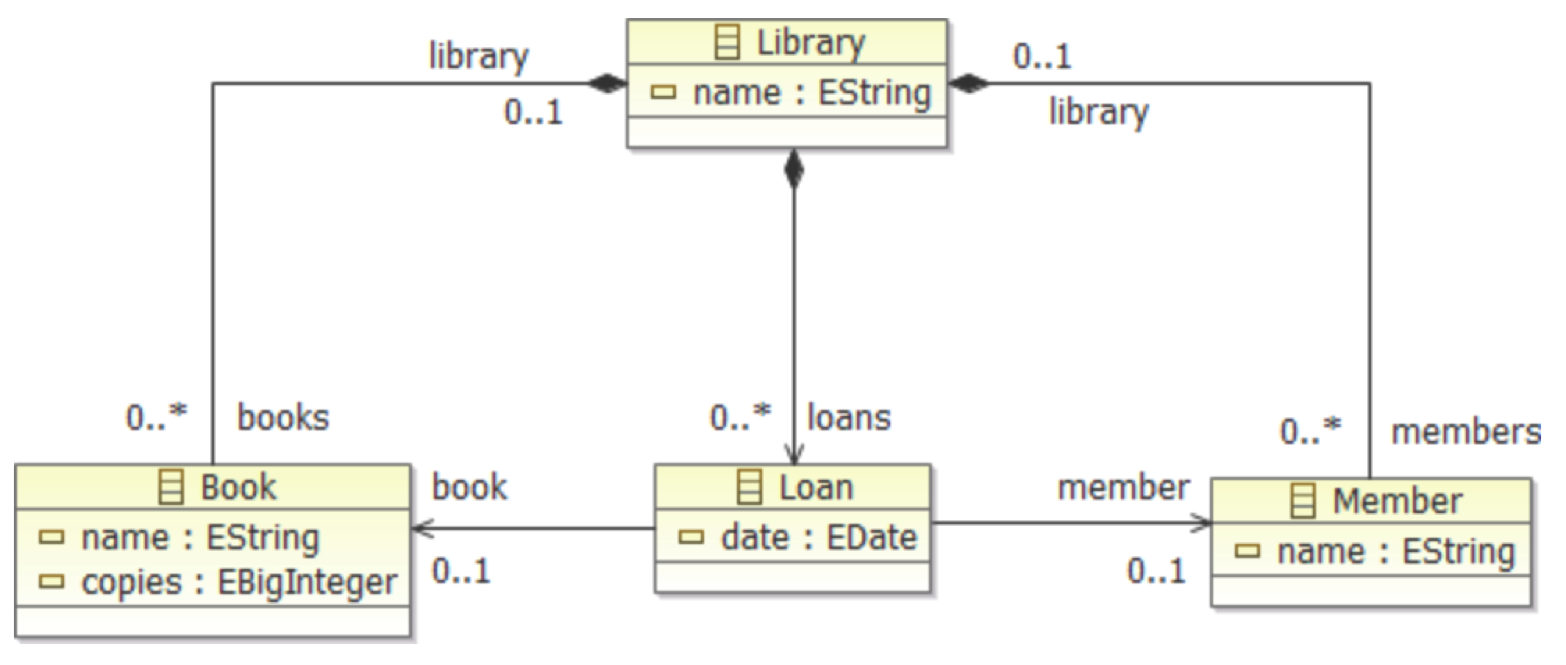
\includegraphics[width=0.9\textwidth]{images/library.png}
\caption{The book library}
\label{fig:library}
\end{figure}

In many modeling situations such diagrams form the core of the modeling effort. Constraints can be added to such diagrams.
For example one constraint could be that the number of copies of a book should be a number bigger than or equal to 1. Such a constraint can be added inside special constraint box on the diagram  in \ref{fig:library}, attached to the \name{Book} box
with a dotted line. It is interesting to note, that such a ``box''
with an associated constraint box conceptually is very similar to
the following Z schema \cite{?}:

\zlang
\begin{lstlisting}
   - Book ----------
   |  name : String
   |  copies : Int
   -----------
   |  copies > 0
   ---------------
\end{lstlisting}

\noindent
This schema represents the fundamental concept of a model: a signature (the declaration of \name{name} and \name{copies} above the line with their types) and then zero or more axioms (below
the line). 
%
The following very similar textual specification is written in
the K specification language \cite{?}, that was developed at JPL
as a textual language for representing class diagrams:

\klang
\begin{lstlisting}
   class Book {
     name : String
     copies : Int
   
     req copies > 0
   }
\end{lstlisting}

\noindent
Let us look more closely at the \name{Book} class. ...

\oclinecore
\begin{lstlisting}
   class Book {
     invariant SufficientCopies:
       library.loans->select(book=self)->size() <= copies;

     attribute name : String;
     attribute copies : Integer;
     property library#books : Library[?];
     
     property loans : Loan[*] { derived }
     {
       derivation: library.loans->select(book=self);
     }

     operation isAvailable() : Boolean[?]
     {
       body: loans->size() < copies;
     }
   }
\end{lstlisting}

\scala
\begin{lstlisting}
   class Book extends Block {
     invariant ("SufficientCopies") {
       library.loans.filter(_.book eq this).size <= copies
     }

     var name: String
     var copies: Integer
     var library: Library

     def loans: Set[Loan] =
       library.loans.filter(_.book eq this)

     def isAvailable(): Boolean =
       loans.size < copies
   }
\end{lstlisting}

\scalaimpl
\begin{lstlisting}
   object Block {
     type Constraint = Unit => Boolean

     var constraints: List[(String, Constraint)] = Nil

     def invariant(c: => Boolean) {
       constraints ::= ("", (Unit => c))
     }

     def invariant(name: String)(c: => Boolean) {
       constraints ::= (name, (Unit => c))
     }

     def evaluate() {
       for ((n, c) <- constraints) assert(c(), n)
     }
   }
\end{lstlisting}


\subsection{VDM Specifications}
\label{sec:vdm-in-scala}

\subsection{Domain Specific Languages}
\label{sec:dsl-in-scala}


